\textbf{3)} As reações paralelas de substituição nucleofílica bimolecular (\ce{Sn 2}) e eliminação bimolecular de formaldeído (\ce{Eco 2}) observadas entre o nitrato de metila (\ce{MeNO3}) e o íon hidróxido foram estudadas e são representadas com suas respectivas constantes de velocidade abaixo:

\begin{align*}
    \ce{MeNO3 + ^-OH &->[{k_{SN 2}}] CH3OH + NO3^-} \\
    \ce{MeNO3 + ^-OH &->[{k_{Eco 2}}] H2O + CH2O + NO2^-}
\end{align*}

Esse estudo experimental foi conduzido a temperatura e pressão constantes e em excesso de nitrato de metila, fornecendo os dados cinéticos a seguir. As reações também foram modeladas do ponto de vista teórico, fornecendo valores de energia relativos dos ``reagentes'' e dos estados de transição, conforme apresentado no diagrama a seguir.

\begin{figure}[H]
    \centering
    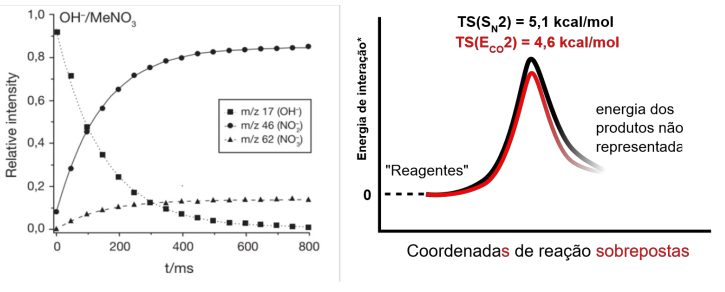
\includegraphics[width=\textwidth]{fig/diagramQ3}
\end{figure}

Considere que os dados teóricos fornecem a estrutura dos reagentes e dos estados de transição abaixo, mas que os valores de energia obtidos possuem uma precisão superior a \qty{1}{\kilo\calorie}.

\begin{figure}[H]
    \centering
    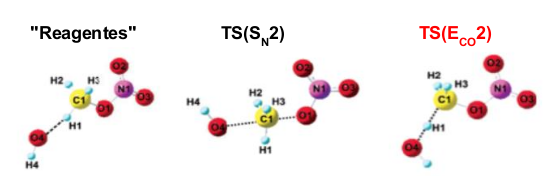
\includegraphics[width=.8\linewidth]{fig/estadosTQ3}
\end{figure}

\textbf{a)} Considerando que a intensidade relativa pode ser considerada como proporcional a concentração dos reagentes, escreva as derivadas \(\frac{d \ce{[HO^-]}}{dt}\), \(\frac{d \ce{[NO3^-]}}{dt}\), \(\frac{ \ce{d[NO2^-]}}{dt}\) em função das constantes de velocidades e das concentrações das espécies envolvidas.

\textbf{Resposta:}

Primeiro, vamos analisar as reações paralelas para cada um dos compostos de interesse. Para \ce{HO^-}, temos que ele é consumido como reagente de ambas as reações. Portanto, a velocidade de consumo de \ce{HO^-} é \(k_{OH} = k_{ \ce{SN 2}} + k_{\ce{Eco 2}}\). Por sua vez, \ce{NO3^-} só é formado por uma reação, então, escrevemos que \(k_{\ce{NO3^-}} = k_{\ce{SN 2}}\). Similarmente, \(k_{\ce{NO2^-}} = k_{\ce{Eco 2}}\). Agora podemos utilizar a lei da velocidade em cada um:

\begin{align*}
    \frac{d \ce{[HO^-]}}{dt} = v_{HO^-} &= - (v_{SN2} + v_{Eco2})\\
                                        &= - k_{OH}[\ce{MeNO3}][\ce{^-OH}]\\
    \frac{d \ce{[NO3^-]}}{dt} = v_{\ce{NO3^-}} &= v_{SN2}\\
                                               &= k_{SN2}[\ce{MeNO3}][\ce{^-OH}]\\
    \frac{d \ce{[NO2^-]}}{dt} = v_{\ce{NO2^-}} &= v_{Eco2}\\
                                               &= k_{Eco2}[\ce{MeNO3}][\ce{^-OH}]
\end{align*}

\commentspace

\textbf{b)} Com os dados cinéticos do gráfico (também apresentados na tabela no fim dessa questão), obtenha a constante de decaimento de \ce{^-OH} experimental, os valores de \ce{k_{SN 2}} e \ce{k_{Eco 2}}.

\textbf{Resposta:}

Como o estudo foi feito com excesso de nitrato de metila, então podemos aproximar que a concentração de nitrato de metila se mantém constante durante toda a reação. Dessa forma, obtemos uma lei de pseudo-primeira ordem. Com isso, sabemos que
\begin{align*}
    \frac{d [HO^-]}{dt} &= -k_{obs} [OH^-] \\
    \implies \int_{[HO^-]_0}^{[HO^-]t} \frac{d[HO^-]}{[HO^-]} &= -k_{obs} \int_0^t dt \\
    \implies \ln |[HO^-]| - \ln|{[HO^-]}_0| &= -k_{obs} t
\end{align*}
. Portanto, podemos computar os valores do log natural utilizando a ferramenta Google Sheets e obter o valor de \(k_{obs} = 5,44 \cdot 10^{-3} \si{\per \milli \second}\). A análise gráfica que resultou neste valor está apresentada na \cref{regressao}.

\begin{figure}[H]
    \centering
    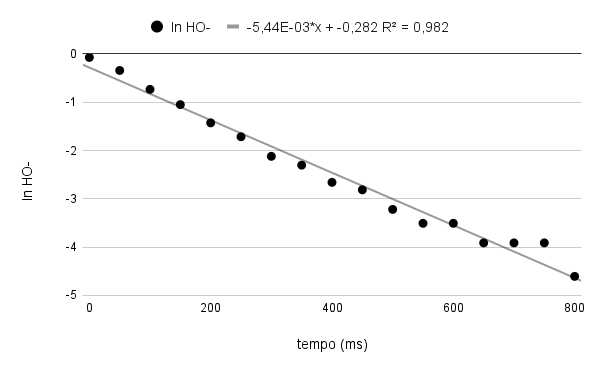
\includegraphics[width=.5\linewidth]{fig/linReg_Q3b}
    \caption{Regressão linear feita com o software Google Sheets. No eixo horizontal estão os valores de tempo em milissegundos. Enquanto, no eixo vertical estão os valores de log natural da intensidade relativa de \ce{HO^-}}\label{regressao}
\end{figure}

Quanto à \(k_{SN2}\), a equação obtida no exercício a) é reduzida à \(\frac{d \ce{[NO3^-]}}{dt} = k_{SN2} [\ce{MeNO3}]_{cte} [^-OH] = k'_{SN2} [^-OH]\). Similarmente, \(\frac{d[\ce{NO2^-}]}{dt} = k_{Eco2}[^-OH]\). Pelos cálculos anteriores, temos que:

\begin{align*}
    \ln [^-OH] - \ln [^-OH]_0 &= -k_{obs}t\\
    \implies [^-OH] &= [^-OH]_0 e^{-k_{obs}t}
\end{align*}

Substituindo \ce{[^-OH]} nas derivadas, obtemos:

\begin{align*}
    \frac{d \ce{[NO3^-]}}{dt} &= k'_{SN2} {[^-OH]}_0 e^{-k_{obs}t} \\
    \implies \int_{[\ce{NO3^-}]_0}^{\ce{[NO3^-]}_t} d \ce{[NO3^-]} &= \int_{0}^{t} k'_{SN2} {[^-OH]}_0 e^{-k_{obs}t} dt \\
    \implies [\ce{NO3^-}] - [\ce{NO3^-}]_0 &= k'_{SN2}[\ce{^-OH}]_0 \frac{e^{-k_{obs}t}}{-k_{obs}} - k'_{SN2} [^-OH]_0 \frac{1}{-k_{obs}} \\
    [NO_3^-] &= \frac{k'_{SN2}[^-OH]_0}{-k_{obs}}(e^{-k_{obs}t} - 1) + [\ce{NO3^-}]_0
\end{align*}

Com isto, é possível obter o valor de \(k_{SN2}\) através da regressão linear dos dados de concentração de \ce{NO3^-} versus \(e^{-k_{obs} t} - 1\). Este processo também foi executado no software Google Sheets e gerou a \cref{reg_NO3}.

\begin{figure}[H]
    \centering
    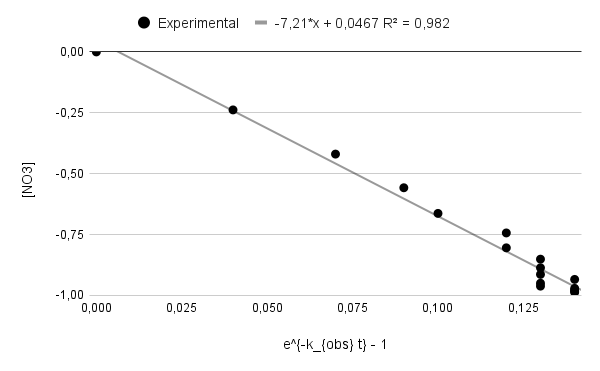
\includegraphics[width=.5\linewidth]{fig/linReg_NO3}
    \caption{Gráfico de dispersão e regressão linear dos dados de concentração de \ce{NO3^-} versus \(e^{-k_{obs} t} - 1\)}\label{reg_NO3}
\end{figure}

Com a equação de reta apresentada na \cref{reg_NO3}, podemos determinar:

\begin{align*}
    \frac{k'_{SN2} [\ce{^-OH}]_0}{-k_obs} = -7,21\\
    \implies k'_{SN2} = \frac{-7,21 \cdot (-5,44 \cdot 10^{-3})}{0,93} = 0.042175 = 42,2 \cdot 10^{-3} \si{\per \milli \second}
\end{align*}

Por fim, para o valor de \(k_{Eco2}\), podemos executar o mesmo processo:

\begin{align*}
    \frac{d[\ce{NO2^-}]}{dt} &= k_{Eco2} [^-\ce{OH}] \\
                             &= k_{Eco2} [^- \ce{OH}]_0 e^{-k_{obs}t}\\
    \implies [\ce{NO2^-}] - [\ce{NO2^-}]_0 &= k_{Eco2} [\ce{^-OH}]_0 \int_{0}^t e^{-k_{obs}t} dt\\
                                           &= \frac{k_{Eco2} [\ce{^-OH}]_0}{-k_{obs}}  (e^{-k_{obs} t} - 1)
\end{align*}

Similarmente ao processo anterior, vamos traçar o gráfico com \ce{[NO2^-]} no eixo y e \(e^{-k_{obs} t} - 1 + \ce{[NO2^-]_0}\) no eixo x. O resultado está exposto na \cref{reg_NO2}.

\begin{figure}[H]
    \centering
    \includegraphics[width=.5\linewidth]{fig/linReg_NO2}
    \caption{Gráfico de dispersão e regressão linear dos dados de concentração de \ce{NO2^-} versus \(e^{-k_{obs}t} -1 + [\ce{NO2^-]_0}\)}\label{reg_NO2}
\end{figure}


Finalmente, para obter o valor de \(k'_{Eco2}\), podemos isolá-lo da expressão obtida para reta:

\begin{align*}
    \frac{k'_{Eco2} [^-\ce{OH}]_0}{-k_{obs}} = -0,77 \\
    \implies k'_{Eco2} = \frac{-0,77 \cdot -5,44 \cdot 10^{-3}}{0,93} = 0.004504 = 4,5 \cdot 10^{-3} \si{\per \milli \second} 
\end{align*}

\commentspace

\textbf{c)} Mostre a partir das derivadas parciais que o valor da constante de decaimento de \ce{^-OH} é igual a soma das outras constantes e mostre que isso se verifica com os valores calculados em b.

\textbf{Resposta:}

Conforme demonstrado no item a):

\begin{align*}
    k_{OH} = k_{SN2} + k_{Eco2} \\
\end{align*}

Disso, temos que:

\begin{align*}
    k_{obs} = k_{OH}[\ce{MeNO3}] = [\ce{MeNO3}] (k_{SN2} + k_{Eco2}) = k'_{SN2} + k'_{Eco2}
\end{align*}

Avaliando numericamente:

\begin{align*}
    k_{obs} = 4,5 \cdot 10^{-3} + 42,2 \cdot 10^{-3} = 46,7 \cdot 10^{-3} \si{\per \milli \second}
\end{align*}

Isso está estranho porque o valor de \(k_{obs}\) obtido anteriormente no gráfico é \(5,44 \cdot 10^{-3} \si{\per\milli\second}\)

\commentspace

A equação de Eyring relaciona o valor da constante de velocidade com a energia livre de ativação, que pode ser representada pela entalpia e entropia de ativação conforme a seguinte equação:

\begin{align*}
    k(T) = \frac{k_b T}{h} e^{\frac{\Delta S^\ddagger}{R}} e^{-\frac{\Delta H^\ddagger}{RT}}   
\end{align*}


\textbf{d)} Considerando que a energia de interação dos estados de transição é praticamente a mesma, dada a precisão dos cálculos teóricos utilizados, explique porque a reação \ce{Eco 2} é mais rápida do que a \ce{SN 2}.

\textbf{Resposta:}

Como a energia de interação dos estados de transição é praticamente a mesma, segue que a variação de entalpia para estes é praticamente a mesma. Segue, observando a equação de Eyring, que é evidente que o termo \(e^{\frac{\Delta S^{\ddagger}}{R}}\) deve ser maior para o Estado de Transição (TS) de Eco2 que de SN2. Estudando os estados de transição propostos, é notável que o TS(Eco2) permite mais movimento conforme o grupo hidroxila atraí um próton da metila enquanto esta se separa do grupo nitrato.

\commentspace

\textbf{e)} Com esses dados, é possível afirmar alguma coisa a respeito do papel do nitrato de metila no mecanismo da reação?

\textbf{Resposta:}

Embora o excesso de nitrato de metila faça a reação se comportar como de pseudo-primeira ordem, os dados corroboram um mecanismo no qual o nitrato de metila participa da etapa elementar lenta de cada reação e cada reação é bimolecular. Ou seja, para ambas as reações, uma molécula de nitrato de metila deve se encontrar com um radical hidroxila para formar o TS e então os produtos. Portanto, sim é possível afirmar que o nitrato de metila atua como participante da etapa lenta de reação e que a reação é de primeira ordem em relação ao nitrato de metila.
Dados cinéticos:

\begin{table}[h]
    \centering
    \caption{Intensidade relativa das espécies}
    \begin{tabular}{c c c c}
        \toprule
        \textbf{tempo/ms} & \textbf{\ce{HO^-}} & \textbf{\ce{NO2^-}} & \textbf{\ce{NO3^-}} \\
        \midrule
        0   & 0,93 & 0,08 & 0,00 \\
        50  & 0,71 & 0,29 & 0,04 \\
        100 & 0,48 & 0,45 & 0,07 \\
        150 & 0,35 & 0,57 & 0,09 \\
        200 & 0,24 & 0,65 & 0,10 \\
        250 & 0,18 & 0,72 & 0,12 \\
        300 & 0,12 & 0,76 & 0,12 \\
        350 & 0,10 & 0,79 & 0,13 \\
        400 & 0,07 & 0,80 & 0,13 \\
        450 & 0,06 & 0,83 & 0,13 \\
        500 & 0,04 & 0,83 & 0,14 \\
        550 & 0,03 & 0,83 & 0,13 \\
        600 & 0,03 & 0,84 & 0,13 \\
        650 & 0,02 & 0,84 & 0,14 \\
        700 & 0,02 & 0,85 & 0,14 \\
        750 & 0,02 & 0,85 & 0,14 \\
        800 & 0,01 & 0,86 & 0,14 \\
        \bottomrule
    \end{tabular}
\end{table}
